%!TEX root = alga.tex
\section{Graphs \`{a} la carte}\label{sec-a-la-carte}

In this section we define several useful \hs{Graph} instances, and
show that the algebra presented in the previous section~\S\ref{sec-algebra} is
not restricted only
to directed graphs, but can be extended to axiomatically represent
undirected~(\S\ref{sub-undirected}), reflexive~(\S\ref{sub-reflexive})
and transitive~(\S\ref{sub-transitive}) graphs, their various
combinations~(\S\ref{sub-preorder}), and even hypergraphs~(\S\ref{sub-hypergraphs}).

\begin{figure*}
\begin{minted}{haskell}
            import           Data.Set (Set, @\blk{singleton, union, elems, fromAscList}@)
            import qualified Data.Set as Set (empty)
\end{minted}
\vspace{1mm}
\begin{minted}{haskell}
            data Relation a = R { domain :: Set a, relation :: Set (a, a) } deriving Eq
\end{minted}
\vspace{1mm}
\begin{minted}{haskell}
            instance Ord a => Graph (Relation a) where
                type Vertex (Relation a) = a
                empty       = R Set.empty Set.empty
                vertex  x   = R (singleton x) Set.empty
                overlay x y = R (domain x `union` domain y) (relation x `union` relation y)
                connect x y = R (domain x `union` domain y) (relation x `union` relation y `union`
                    fromAscList [ (a, b) | a <- elems (domain x), b <- elems (domain y) ])
\end{minted}
\vspace{-2mm}
\caption{Implementing the \hs{Graph} type class by a binary relation
and the core graph construction primitives
defined in~\S\ref{sub-constructing}.\label{fig-relation}}
\vspace{-2mm}
\end{figure*}

\subsection{Binary relation}\label{sub-relation}

We start by a direct encoding of the graph construction primitives defined
in~\S\ref{sub-constructing} into the abstract data type \hs{Relation} isomorphic
to a pair of sets $(V,E)$, see Fig.~\ref{fig-relation}. As we have seen,
this implementation satisfies the axioms of the graph algebra. Furthermore, it
is a \emph{free graph} in the sense that it does not satisfy any other laws.
This follows from the fact that any algebraic graph expression $g$ can be
rewritten in the following \emph{canonical form}:
\[
g = \Big(\sum_{v\in V_g} v\Big) + \Big(\sum_{(u,v)\in E_g} \hspace{-1mm} u \rightarrow v\Big),
\]
\noindent
where $V_g$ is the set of vertices that appear in $g$, and $(u,v)\in E_g$ if
vertices $u$ and $v$ appear in the left-hand and right-hand arguments of
the connect operation $\rightarrow$ at least once (and should thus be connected
by an edge). The canonical form of an
expression $g$ can be represented as \hs{R@$\,\,V_g\,E_g$@}, and any additional
law on \hs{Relation} would therefore violate the canonicity property.
The existence of the canonical form was proved by~\citet{2014_algebra_mokhov}
for an extended version of the algebra. The proof fundamentally builds on the
decomposition axiom: one can apply it repeatedly to an expression, breaking up
connect sequences $x\rightarrow y\rightarrow z$ into pairs $x \rightarrow y$
until the decomposition can no longer be applied. We can then open parentheses,
such as $x\rightarrow (y + z)$, using the distributivity axiom and rearrange
terms into the canonical form by the commutativity and idempotence of overlay~$+$.

It is convenient to make \hs{Relation} an instance of the \hs{Num} type class
to use the standard $+$ and $*$ operators as shortcuts for \hs{overlay} and
\hs{connect}, respectively:

\begin{minted}{haskell}
instance (Ord a, Num a) => Num (Relation a) where
    fromInteger = vertex . fromInteger
    (+)         = overlay
    (*)         = connect
    signum      = const empty
    abs         = id
    negate      = id
\end{minted}

\noindent
Note that the \hs{Num} law \hs{@\blk{abs}@ x * signum x == x} is satisfied by the above
definition since $x \rightarrow \varepsilon = x$. Any \hs{Graph} instance
can be made a \hs{Num} instance if need be, using a definition similar to the above.

We can now experiment with graphs and binary relations using the interactive GHC:

\begin{minted}[frame=single,fontsize=\small]{haskell}
@\ghci@ 1 * (2 + 3) :: Relation Int
R@\,@{domain@\,@=@\,\blk{fromList}\,@[1,2,3],@\,\blk{relation}\,@=@\,\blk{fromList}\,@[(1,2),(1,3)]}
@\ghci@ 1 * (2 + 3) + 2 * 3 == (clique [1..3] :: Relation Int)
True
@\ghci@ 1 * 2 == (2 * 1 :: Relation Int)
False
\end{minted}
\begin{minted}[frame=single,fontsize=\small]{haskell}
@\ghci \blk{:t}@ clique "abc"
clique "abc" :: (Graph g, Vertex g @\teq@ Char) => g
@\ghci @relation (clique "abc")
fromList [('a','b'),('a','c'),('b','c')]
\end{minted}

\noindent
The last example highlights the fact that the \hs{Relation@\,\,\blk{a}@} instance allows vertices
of any type \hs{@\blk{a}@} that satisfies the~\hs{Ord@\,\,\blk{a}@} constraint.

\subsection{Deep embedding}\label{sub-embedding}

We can embed the core graph construction primitives into a simple data type
(excuse and ignore the name clash with the type class):

\begin{minted}{haskell}
data Graph a = Empty
             | Vertex a
             | Overlay (Graph a) (Graph a)
             | Connect (Graph a) (Graph a)
\end{minted}

The instance definition is a direct mapping from the \emph{shallow embedding}
of the core primitives, represented by the type class, into the
corresponding \emph{deep embedding}, represented by the data type.
It is known, e.g. see~\citet{2014_gibbons_folding}, that by \emph{folding} the data
type one can always obtain the inverse mapping:

\begin{minted}{haskell}
fold :: Graph g => Graph (Vertex g) -> g
fold Empty         = empty
fold (Vertex  x  ) = vertex x
fold (Overlay x y) = overlay (fold x) (fold y)
fold (Connect x y) = connect (fold x) (fold y)
\end{minted}

We cannot use the derived \hs{Eq} instance of the \hs{Graph} data type, because it
would clearly violate the axioms of the algebra, e.g. \hs{Overlay@\,\,@Empty@\,\,@Empty} is
structurally different from \hs{Empty}, but they must be equal according to the axioms.
One way to implement a custom law-abiding \hs{Eq} instance is to \emph{reinterpret}
the graph expression as a binary relation, thereby gaining access to the canonical
graph representation:

\begin{minted}{haskell}
instance Ord a => Eq (Graph a) where
    x == y = fold x == (fold y :: Relation a)
\end{minted}

An interesting feature of this graph instance is that it allows to represent
densely connected graphs more compactly. For example, \hs{clique [1..n] :: Graph Int}
has a linear-size representation in memory, while \hs{clique [1..n] :: Relation Int}
stores each edge separately and therefore requires $O(n^2)$ memory. Exploiting the
compact graph representation for deriving algorithms that are asymptotically faster
on dense graphs, compared to conventional algorithms operating on `uncompressed'
graph representations isomorphic to $(V,E)$, is outside the scope of this paper,
but is an interesting direction of future research.

% \begin{figure*}
% \begin{minted}{haskell}
% import           Data.Map.Strict (Map, keysSet, fromSet)
% import qualified Data.Map.Strict as Map
% import           Data.Set (Set)
% import qualified Data.Set as Set
% \end{minted}
% \vspace{1mm}
% \begin{minted}{haskell}
% newtype AdjacencyMap a = AM { adjacencyMap :: Map a@\,\,@(Set a) }@\,\,@deriving@\,\,@(Arbitrary,@\,\,@Eq,@\,\,@Show)
% \end{minted}
% \vspace{1mm}
% \begin{minted}{haskell}
% instance Ord a => Graph (AdjacencyMap a) where
%     type Vertex (AdjacencyMap a) = a
%     empty       = AM $ Map.empty
%     vertex  x   = AM $ Map.singleton x Set.empty
%     overlay x y = AM $ Map.unionWith Set.union (adjacencyMap x) (adjacencyMap y)
%     connect x y = AM $ Map.unionsWith Set.union [ adjacencyMap x, adjacencyMap y,
%         fromSet (const . keysSet $ adjacencyMap y) (keysSet $ adjacencyMap x) ]
% \end{minted}
% \caption{Implementing the \hs{Graph} type class by adjacency map\label{fig-adjacency-map}}
% \end{figure*}

% \subsection{Adjacency map and friends}\label{sub-adjacency-map}

% In this subsection we show how to reuse existing graph libraries, such as
% \textsf{containers} and \textsf{fgl}, by wrapping them into the algebraic
% graph API. More specifically, we show how to reuse the efficient implementations
% of the \emph{depth-first search forest} and \emph{topological sort} algorithms
% developed by~\citet{1995_king_graphs}.

% The interface of the \textsf{containers} library uses the \emph{adjacency list}
% representation of graphs and we therefore define a new \hs{Graph} instance that
% provides the closest match, see Fig.~\ref{fig-adjacency-map}. In our experiments
% this instance is often faster than \hs{Relation} because of more efficient
% sharing of common subgraphs in memory, see benchmarks in~\S\ref{sub-library-summary}.

% The \hs{AdjacencyMap} instance is parametric and in order to use the
% functions provided by \textsf{containers}, we need to map the graph vertices
% into a contiguous subset of integers \hs{Int}. This can be done by the
% \hs{graphFromEdges} function provided by \textsf{containers} that takes an adjacency
% list as the input. We can obtain the adjacency list from the \hs{AdjacencyMap}
% instance:

% \begin{minted}{haskell}
% adjacencyList :: AdjacencyMap a -> [(a, [a])]
% adjacencyList = @\std{map}@ (@\std{fmap}@ Set.toAscList) . Map.toAscList . adjacencyMap
% \end{minted}
% Both \textsf{containers} and \textsf{fgl} also provide graph constructors from
% \emph{edge lists}, which we compute as follows:

% \begin{minted}{haskell}
% edgeList :: AdjacencyMap a -> [(a, a)]
% edgeList = @\std{concatMap}@ (\(x, ys) -> @\std{map}@ (x,) ys) . adjacencyList
% \end{minted}

% \noindent
% Let's test that \hs{AdjacencyMap} is a valid \hs{Graph} instance and
% showcase \hs{adjacencyList} and \hs{edgeList}:

% @\ghci @quickCheck (axioms :: GraphTestsuite (AdjacencyMap Int))
% @\blk{+++ OK, passed 100 tests.}@
% \begin{minted}[frame=single]{haskell}
% @\ghci @adjacencyList $ clique [1..4]
% [(1,[2,3,4]),(2,[3,4]),(3,[4]),(4,[@@])]

% @\ghci @edgeList $ edges [('a','b'),('b','c'),('a','b')]
% [('a','b'),('b','c')]
% \end{minted}

% We can now build bridges to \textsf{containers} and \textsf{fgl}. For example,
% the following are safe and parametric interfaces to depth-first
% search forest and topological sort algorithms (we do not show the underlying plumbing):

% \begin{minted}{haskell}
% dfsForest :: Ord a => AdjacencyMap a -> Forest a  -- uses Data.Graph.dff
% topSort   :: Ord a => AdjacencyMap a -> Maybe [a] -- uses Data.Graph.topSort
% \end{minted}

% \noindent
% Note the return type of \hs{topSort}: the function returns \hs{Nothing}
% if the graph is cyclic and no topological sort exists; otherwise it
% returns a list of vertices in the topological order, as demonstrated below.

% \begin{minted}[frame=single]{haskell}
% @\ghci @topSort $ 1 * 2 + 3 * 1
% Just [3,1,2]

% @\ghci @topSort $ 1 * 2 + 2 * 1
% Nothing
% \end{minted}

% Consider the following interesting
% wrapper\footnote{We use \textsf{GeneralizedNewtypeDeriving} GHC
% extension to derive \hs{Arbitrary}, \hs{Graph} and \hs{Num} instances. Note that
% the current version of GHC does not support the extension for classes
% with associated types, such as \hs{Graph}, but the feature has already been
% implemented (ticket \#8165) and will be available in the next GHC release.
% Until then one needs to write the trivial \hs{Graph} instance manually.}
% around \hs{AdjacencyMap}:

% \begin{minted}{haskell}
% newtype TopSort a = TS (AdjacencyMap a) deriving (Arbitrary, Graph, Num, Show)
% \end{minted}
% \vspace{1mm}
% \begin{minted}{haskell}
% instance Ord a => Eq (TopSort a) where
%     TS x == TS y = topSort x == topSort y
% \end{minted}

% \noindent
% \hs{TopSort} differs from \hs{AdjacencyMap} only in one aspect: it uses
% a custom equality test, which satisfies \emph{more} laws than required by the \hs{Graph}
% instance. Indeed, there are many pairs of different graphs, whose topological sorts
% coincide, e.g. \hs{topSort (1 + 2)} $=$ \hs{topSort (1 * 2)} $=$ \hs{Just [1,2]}.
% A similar \hs{newtype DfsForest} can be created for the depth-first search
% forest algorithm. It will also trivially satisfy the \hs{Graph} axioms, but will have
% a different equivalence relation, since \hs{dfsForest (1 + 2)} $\neq$ \hs{dfsForest (1 * 2)}.
% These examples demonstrate that the world of \hs{Graph} instances is rich and complex,
% which motivates us to study polymorphic graph transformations that can be reused by
% all law-abiding citizens of the \hs{Graph} world -- see \S\ref{sec-transformations}.

\subsection{Undirected graphs}\label{sub-undirected}

As hinted in \S\ref{sub-laws}, to switch from directed to undirected graphs it
is sufficient to add the axiom of commutativity for the connect operation. For
undirected graphs we can denote connect by $\leftrightarrow$:

\begin{itemize}
    \item $\leftrightarrow$ is commutative: $x \leftrightarrow y = y \leftrightarrow x$.
\end{itemize}

Curiously, with the introduction of this axiom, the associativity of $\leftrightarrow$
follows from the left-associated version of the decomposition axiom and the
commutativity of $+$:
\[
\begin{array}{rcll}
(x \leftrightarrow y) \leftrightarrow z & = & x \leftrightarrow y + x \leftrightarrow z + y \leftrightarrow z & \text{(decomposition)}\\
 & = & y \leftrightarrow z + y \leftrightarrow x + z \leftrightarrow x & \text{(commutativity)}\\
 & = &  (y \leftrightarrow z) \leftrightarrow x & \text{(decomposition)}\\
 & = &   x \leftrightarrow (y \leftrightarrow z) & \text{(commutativity)}\\
\end{array}
\]

Therefore, \emph{the minimal algebraic characterisation of undirected graphs}
comprises only 6 axioms:

\begin{itemize}
    \item $+$ is commutative and associative, i.e. $x + y = y + x$ and
    $x + (y + z) = (x + y) + z$.
    \item $\leftrightarrow$ is commutative $x \leftrightarrow y = y \leftrightarrow x$ and
    has $\varepsilon$ is the identity: $x \leftrightarrow \varepsilon = x$.
    \item Left distributivity:
    $x \leftrightarrow (y + z) = x \leftrightarrow y + x \leftrightarrow z$.
    \item Left decomposition: $(x \leftrightarrow y) \leftrightarrow z =
    x \leftrightarrow y + x \leftrightarrow z + y \leftrightarrow z$.
\end{itemize}

Commutativity of the connect operator forces graph expressions that differ only
in the direction of edges into the same equivalence class. One can implement
this by the \emph{symmetric closure} of the underlying binary relation:

\begin{minted}{haskell}
newtype Symmetric a = S@\,@(Relation a)@\,@deriving@\,@(Graph,@\,@Num)
\end{minted}
\vspace{1mm}
\begin{minted}{haskell}
instance Ord a => Eq (Symmetric a) where
    S@\,\blk{x}@ == S@\,\blk{y}@ = symmetricClosure@\,\blk{x}@ == symmetricClosure@\,\blk{y}@
\end{minted}

Note that algebraic expressions of undirected graphs have the canonical form where all
edges are directed in a canonical order, e.g. according to some total order on vertices.

Let's test that the custom equality works as desired:
% @\ghci @quickCheck (axioms :: GraphTestsuite (Symmetric Int))
% @\blk{+++ OK, passed 100 tests.}@

% @\ghci @quickCheck $ \x y -> x * y == (y * x :: Symmetric Int)
% @\blk{+++ OK, passed 100 tests.}@
\begin{minted}[frame=single,fontsize=\small]{haskell}
@\ghci @clique "abcd" == (clique "dcba" :: Relation Char)
False

@\ghci @clique "abcd" == (clique "dcba" :: Symmetric Char)
True
\end{minted}

As you can see, polymorphic graph construction functions, such as \hs{clique},
can be reused when working with undirected graphs. We can define a subclass
\hs{class Graph@\,\,\blk{g}@ => UndirectedGraph@\,\,\blk{g}@} and use the
\hs{UndirectedGraph@\,\,\blk{g}@}
constraint for functions that rely on the commutativity of the \hs{connect} method.

\begin{figure*}
\centerline{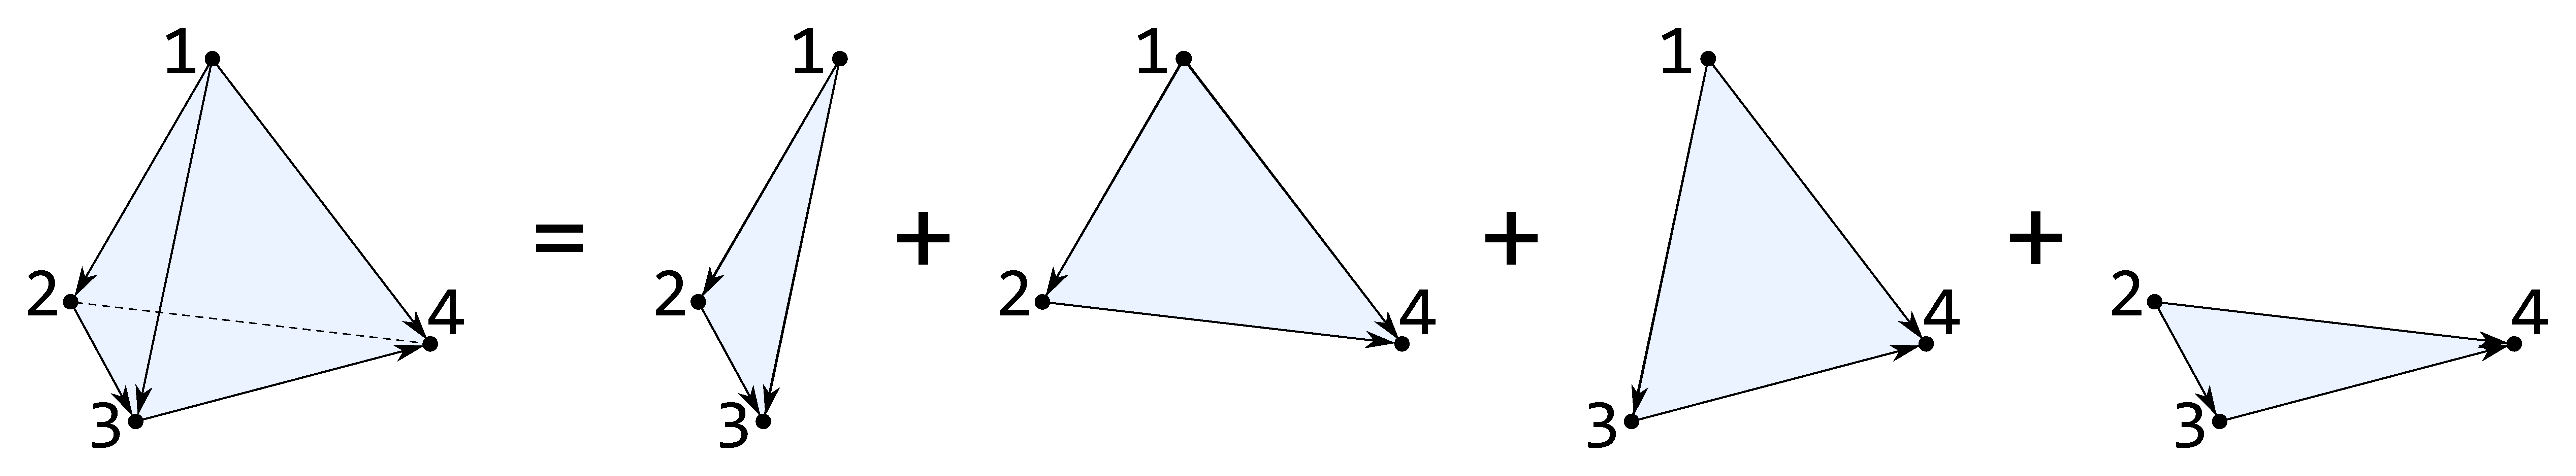
\includegraphics[scale=0.12]{fig/3-decomposition.pdf}}
\caption{3-decomposition:
    $1 \rightarrow 2 \rightarrow 3 \rightarrow 4 =
    1 \rightarrow 2 \rightarrow 3 + 1 \rightarrow 2 \rightarrow 4 +
    1 \rightarrow 3 \rightarrow 4 + 2 \rightarrow 3 \rightarrow 4$.
    \label{fig-3-decomposition}}
\end{figure*}

\subsection{Reflexive graphs}\label{sub-reflexive}

A graph is \emph{reflexive} if every vertex of the graph is connected to itself,
i.e. has a self-loop. An example of a reflexive graph is the graph corresponding
to the partial order relation $\subseteq$ on graphs: indeed, $x \subseteq x$ holds
for all $x$. To represent reflexive graphs algebraically we can introduce the
following axiom:

\begin{itemize}
    \item Self-loop: $v = v \rightarrow v$, where $v\in \mathbb{V}$ is a vertex.
\end{itemize}

\noindent
The self-loop axiom corresponds to the additional \hs{Graph} law:

\begin{itemize}
    \item \hs{vertex x} = \hs{connect (}\hs{vertex x) (}\hs{vertex x)}.
\end{itemize}

One can implement the reflexive \hs{Graph} instance analogously to the
implementation of the \hs{Symmetric} data type presented in~\S\ref{sub-undirected},
by wrapping the \hs{Relation} into a \hs{newtype} and giving it a custom \hs{Eq}
instance based on the \hs{reflexiveClosure}.

We can define
\hs{class Graph@\,\,\blk{g}@ => ReflexiveGraph@\,\,\blk{g}@}
to increase the type safety of functions that rely on the self-loop axiom.

\subsection{Transitive graphs}\label{sub-transitive}

In many applications graphs satisfy the \emph{transitivity} property: if a vertex $x$ is
connected to $y$, and $y$ is connected to $z$, then the edge between $x$ and $z$ can be
added or removed without changing the semantics of the graph. A common example is
\emph{dependency graphs} or \emph{partial orders} --- the semantics of such graphs is
typically their \emph{transitive closure}.
To describe this class of graphs algebraically we add the following \emph{closure} axiom:

\begin{itemize}
    \item Closure: $y \neq \varepsilon \Rightarrow x \rightarrow y + y \rightarrow z +
    x \rightarrow z = x \rightarrow y + y \rightarrow z$.
\end{itemize}

By using the axiom one can rewrite a graph expression into its transitive closure or,
alternatively, into its \emph{transitive reduction}, hence all graphs that differ only in the
existence of some transitive edges are forced into the same equivalence class. Note that the
precondition $y \neq \varepsilon$ is necessary as otherwise $+$ and $\rightarrow$ can no
longer be distinguished, which is clearly undesirable:
\[
x\!\rightarrow\!z = x\!\rightarrow\!\varepsilon\!\rightarrow z = x\!\rightarrow\!\varepsilon
 + \varepsilon\!\rightarrow\!z + x\!\rightarrow\!z = x\!\rightarrow\!\varepsilon
 + \varepsilon\!\rightarrow\!z = x + z.
\]

It is interesting to note that $+$ and $\rightarrow$ have simple meanings for transitive
graphs: they correspond to the \emph{parallel} and \emph{sequential composition},
respectively. This allows to algebraically describe concurrent systems, which was
the original motivation behind the research on algebraic graphs~\cite{2014_algebra_mokhov}.

We can implement transitive graphs by wrapping
\hs{Relation} in a \hs{newtype Transitive} with a custom equality test that
compares the transitive closures of the underlying relations.
A subclass \hs{class Graph@\,\,\blk{g}@ => TransitiveGraph@\,\,\blk{g}@} can be
defined to distinguish algebraic graphs with the closure axiom from others.

\subsection{Preorders and equivalence relations}\label{sub-preorder}

By combining reflexive and transitive graphs, one can obtain \emph{preorders}.
For example, $(1 + 2 + 3) \rightarrow (2 + 3 + 4)$
is a preorder with vertices 2 and 3 forming a \emph{strongly-connected component}. By
finding all strongly-connected components in the graph (e.g. by utilising the
function \hs{scc} from the \textsf{containers} library) we can derive the
following \emph{graph condensation}:
$\{1\} \rightarrow \{2, 3\} \rightarrow \{4\}$. One way to interpret this preorder as a
dependency graph is that tasks 2 and 3 are executed as a step, simultaneously,
and that they both depend on task 1, and are prerequisite for task 4. Note that
having sets as the type of graph vertices is perfectly legal: the type of the
above graph condensation is \hs{(Graph g, Vertex g @\teq@ Set Int) => g}.

One can further combine preorders and undirected graphs, obtaining \emph{equivalence
relations}, which can be equipped with an efficient instance based on the
\emph{disjoint set} data structure~\cite{1984_set_union_tarjan}. One interesting
application of the resulting algebra is modelling connectivity in
circuits~\cite{2015_mokhov_algebra}.

\subsection{Hypergraphs}\label{sub-hypergraphs}

As described in~\S\ref{sub-relation}, the decomposition axiom collapses an algebraic
graph expression into a collection of vertices and pairs of vertices (i.e. graphs).
By replacing the decomposition axiom with \emph{3-decomposition}, we obtain
\emph{hypergraphs} comprising vertices, edges and \emph{3-edges} (triples of vertices):

\begin{itemize}
    \item 3-decomposition: $w \rightarrow x \rightarrow y \rightarrow z = \\
    w \rightarrow x \rightarrow y + w \rightarrow x \rightarrow z +
    w \rightarrow y \rightarrow z + x \rightarrow y \rightarrow z$.
\end{itemize}

Fig.~\ref{fig-3-decomposition} illustrates the axiom by decomposing a tetrahedron
into four 3-edges corresponding to its \emph{faces}. To better understand the
difference between the (2-)decomposition and 3-decomposition
axioms, let us substitute~$\varepsilon$ for $w$ in the 3-decomposition and simplify:
\[
x \rightarrow y \rightarrow z = x \rightarrow y + x \rightarrow z + y \rightarrow z
+ x \rightarrow y \rightarrow z.
\]
This is almost the 2-decomposition axiom, yet there is no way to get rid
of the term $x \rightarrow y \rightarrow z$ on the right-hand side: indeed, a triple is
unbreakable
in this algebra, and one can only extract the pairs (edges) that are embedded in it.
In fact, we can take this further and rewrite the above expression to also expose the
embedded vertices:
\[
x \rightarrow y \rightarrow z = x + y + z + x \rightarrow y + x \rightarrow z
+ y \rightarrow z + x \rightarrow y \rightarrow z.
\]
Note that with 2-decomposition we can achieve something similar via the absorption theorem:
\[
x \rightarrow y = x + y + x \rightarrow y.
\]
This can be taken further by defining 4-decomposition and so forth, creating a hierarchy
of algebraic structures corresponding to hypergraphs of different ranks.

Since every graph is also a hypergraph, we can define a superclass
\hs{class HyperGraph@\,\,\blk{g}@ => Graph@\,\,\blk{g}@}, moving all \hs{Graph} methods to the superclass, and
leaving only the decomposition axiom in \hs{Graph}, as the law that distinguishes it from
\hs{HyperGraph}.

% \subsection{Summary}

% In this section we have defined a family of graph instances and their classes that
% build on the algebraic core presented in~\S\ref{sec-algebra}. The additional axioms
% that characterise these classes
% can be mixed in various combinations. As an example, the algebra of undirected, reflexive
% and transitively closed graphs describes the laws of \emph{equivalence} relations and can be
% equipped with an
% efficient instance based on the \emph{disjoint set} data structure~\cite{1984_set_union_tarjan}.

% In the next section we present a library of basic graph transformation algorithms that
% can be reused by all graph instances discussed in this section.
